\chapter{Debugger}
\label{chap:debugger}
In diesem Kapitel wird beschrieben, wie der Debugger in Eclipse integriert wurde. Es wird aufgezeigt, welche Möglichkeiten existieren, einen Debugger in Eclipse zu integrieren und welche dieser Möglichkeiten implementiert wurden.

\section{Breakpoints}
Als erstes müssen für den Debugger Breakpoints gesetzt werden können. Dafür stehen zwei Möglichkeiten zur Verfügung, die in den nächsten Kapiteln erläutert und verglichen werden.

\subsection{Per Konsole}

Breakpoints können per Konsole gesetzt werden. Das Senden der Befehle funktioniert mit den im Kapitel \ref{chap:forthcommunication} beschriebenen Klassen. In der Konsole kann der Befehl

%
\begin{verbatim}
debug _function
\end{verbatim}
%
eingegeben werden, um einen Breakpoint zu setzen. Wobei \verb!_function! für eine beliebige Forth Funktion steht.

\subsection{Im Source Code}

Breakpoints können im C-File gesetzt werden. Dies wurde so realisiert, dass der Breakpoint nur auf eine Funktionsdefinition gesetzt werden kann. Alle anderen Zeilen des C-Source Codes können nicht direkt auf den übersetzten Forth Code abgebildet werden und sind deshalb nicht erlaubt für die Breakpoints.
\newline
Eclipse-CDT stellt den Abstract Synatx Tree (AST) des C-Files zur Verfügung. Mit Hilfe des AST kann überprüft werden, ob sich der Breakpoint wirklich auf einer Funktionsdefinition befindet.
\newpage
\section{Konsolenbasierter Debugger}

Eine einfache Integration des Debuggers besteht in der Verwendung, des Konsolen Debugger von Forth im Eclipse. Dieser kann mit den im Kapitel \ref{chap:forthcommunication} beschriebenen Kommunikationsmitteln angesteuert und in einer Eclipse Console View angezeigt werden.

\begin{figure}[H]
	\centering
		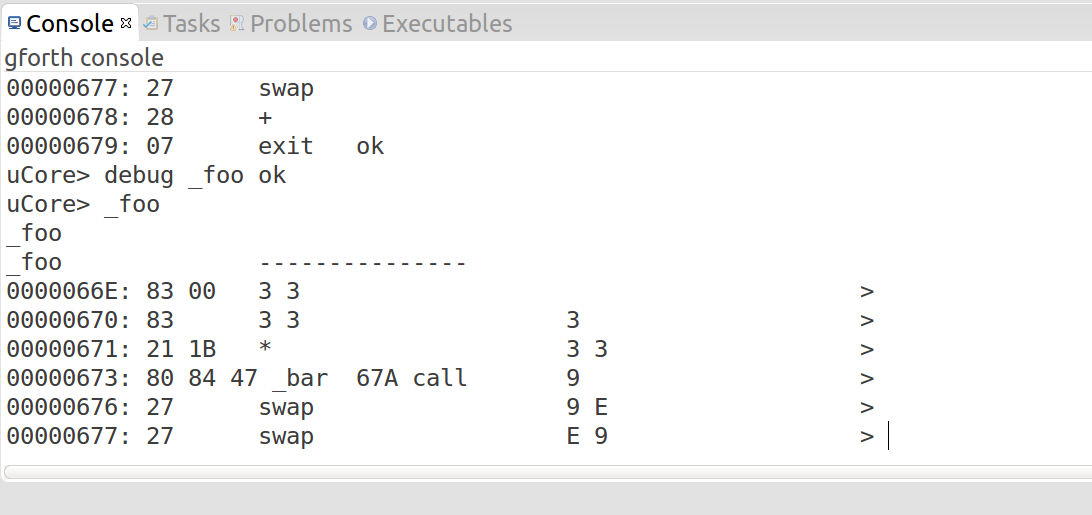
\includegraphics[scale=0.35]{debugger/consoledebugger.png}
		\caption{Konsolenbasierter Debugger. Der Debugger kann über die Eclipse Console View gesteuert werden.}
		\captionsetup{margin=0cm,font={footnotesize}}
		\label{fig:consoledebugger}
\end{figure}

\section{Forth Debugger}

Eine weitere Möglichkeit besteht darin, das Debug User Interface von Eclipse zu verwenden, um den Debugger zu steuern. Dies ist für den Anwender angenehmer, da alle Informationen des Debuggers in einem User Interface ersichtlich sind.

\subsection{CDT oder JDT Debugging-Mechanismen}

Eclipse stellt mehrere Möglichkeiten zur Verfügung, einen Debugger zu integrieren. Es können die Mechanismen vom Eclipse JDT (insbesondere das Plugin \verb!org.eclipse.debug.core!) verwendet werden oder die erweiterten Mechanismen von CDT (insbesondere das Plugin \verb!org.eclipse.cdt.debug.core!) mit denen C oder C++ Debugger integriert werden. Das vom CDT zur Verfügung gestellte Plugin wird vor allem dazu verwendet, um einen neuen C oder C++ Debugger zu integrieren. Da es sich aber um einen Forth Debugger handelt, werden diese Erweiterungen nicht gebraucht. Ich habe mich deshalb dazu entschieden, die Eclipse JDT Debugging-Mechanismen zu verwenden.

\subsection{Debugger-Aktionen}

Für den Debugger wurden einige Aktionen, die schon in Eclipse verwendet werden, implementiert und einige neue Forth-spezifische Aktionen hinzugefügt.

\subsubsection{Resume}

Mit der Resume-Aktion kann der Prozess während des Debuggens fortgeführt werden. Dafür wird ein \verb!end-trace! Befehl an den Forth-Prozess gesendet. Der \verb!end-trace! Befehl entfernt auch alle Breakpoints. Diese werden von der Resume-Aktion automatisch nach der Ausführung neu gesetzt. 

\begin{figure}[H]
	\centering
		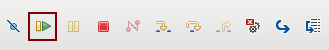
\includegraphics[scale=1]{debugger/resume.png}
		\caption{Resume-Aktion.}
		\captionsetup{margin=0cm,font={footnotesize}}
		\label{fig:resume}
\end{figure}

\subsubsection{Terminate}

Mit der Terminate-Aktion kann der Prozess heruntergefahren werden, indem der \verb!bye! Befehl gesendet wird. Falls der Prozess nicht mehr reagiert, sollte die Kill-Aktion verwendet werden. Die Terminate Aktion unterscheidet sich von der Kill-Aktion, in dem sie versucht den Prozess auf normale Weise zu beenden und nicht über ein Kill-Signal.

\begin{figure}[H]
	\centering
		
\includegraphics[scale=1]{debugger/terminate.png}
		\caption{Terminate-Aktion.}
		\captionsetup{margin=0cm,font={footnotesize}}
		\label{fig:terminate}
\end{figure}

\subsubsection{Step Into}

Mit der Step-Into-Aktion kann in eine Funktion gesprungen werden, falls die nächste Zeile ein Funktionsaufruf ist. Dafür wird ein \verb!nest! Befehl an den Forth-Prozess gesendet.

\begin{figure}[H]
	\centering
		
\includegraphics[scale=1]{debugger/stepinto.png}
		\caption{Step-Into-Aktion.}
		\captionsetup{margin=0cm,font={footnotesize}}
		\label{fig:stepinto}
\end{figure}

\newpage

\subsubsection{Step}

Mit der Step-Aktion kann ein Single Step ausgeführt werden. Dafür wird ein \verb!CR! Befehl an den Forth-Prozess gesendet.

\begin{figure}[H]
	\centering
		
\includegraphics[scale=1]{debugger/step.png}
		\caption{Step-Aktion.}
		\captionsetup{margin=0cm,font={footnotesize}}
		\label{fig:step}
\end{figure}

\subsubsection{Kill}

Mit der Kill-Aktion kann der Prozess terminiert werden, in dem das Kill-Signal gesendet wird. Im Normalfall sollte die Terminate-Aktion verwendet werden, da sie den Forth-Prozess über den \verb!bye! Befehl beendet.

\begin{figure}[H]
	\centering
		
\includegraphics[scale=1]{debugger/kill.png}
		\caption{Kill Aktion.}
		\captionsetup{margin=0cm,font={footnotesize}}
		\label{fig:kill}
\end{figure}

\subsubsection{After}

Die After-Aktion setzt den Breakpoint nach der nächsten Instruktion, falls es sich um einen Rückwärtssprung handelt, welcher möglicherweise von einer 
\verb!UNTIL!-, \verb!REPEAT!-, \verb!LOOP!- oder \verb!NEXT!-Instruktion kompiliert wurde. Der Rest der Schleife wird deshalb ohne Unterbruch ausgeführt.

\begin{figure}[H]
	\centering
		
\includegraphics[scale=1]{debugger/after.png}
		\caption{After-Aktion.}
		\captionsetup{margin=0cm,font={footnotesize}}
		\label{fig:after}
\end{figure}

\subsubsection{Jump}

Mit der Jump-Aktion kann über die nächste auszuführende Instruktion gesprungen werden. Dafür wird ein \verb!jump! Befehl an den Forth Prozess gesendet.

\begin{figure}[H]
	\centering
		
\includegraphics[scale=1]{debugger/jump.png}
		\caption{Jump-Aktion.}
		\captionsetup{margin=0cm,font={footnotesize}}
		\label{fig:jump}
\end{figure}

\newpage

\subsection{Stack View}

In der Stack View wird der aktuelle Data-Stack angezeigt. Die Stack View wird automatisch nach jedem Steppen des Debuggers aktualisiert.

\begin{figure}[H]
	\centering
		
\includegraphics[scale=0.35]{debugger/stack.png}
		\caption{Stack View mit aktuellem Inhalt des Dstacks. Der Top Of Stack (TOS) befindet sich zuoberst in der Liste.}
		\captionsetup{margin=0cm,font={footnotesize}}
		\label{fig:stack}
\end{figure}


\subsection{Memory View}

In der Memory View kann ein Memory Dump, der mit dem \verb!dump!-Befehl von uForth abgefragt wird, angezeigt werden. Der Memory Dump wird automatisch nach jedem Steppen des Debuggers aktualisiert.

\begin{figure}[H]
	\centering
		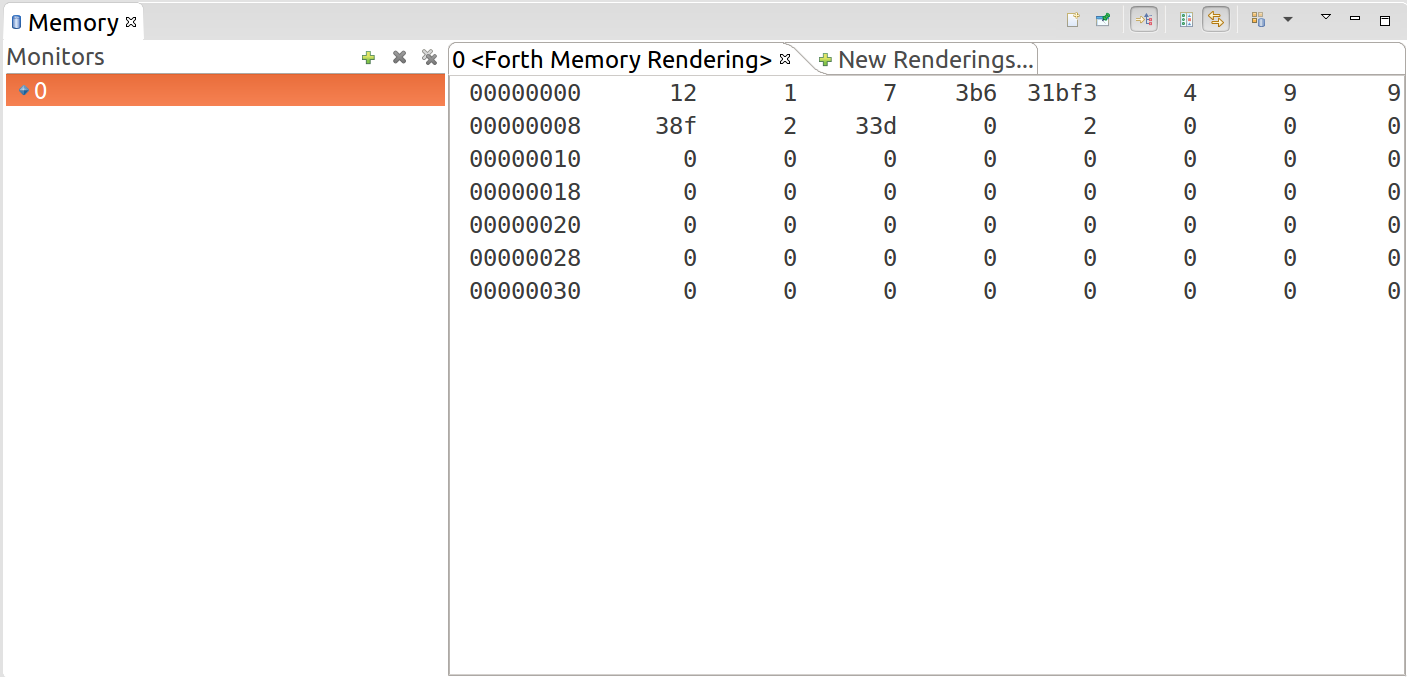
\includegraphics[scale=0.35]{debugger/dump.png}
		\caption{Die Memory View mit dem Inhalt eines dump-Befehls.}
		\captionsetup{margin=0cm,font={footnotesize}}
		\label{fig:dump}
\end{figure}


\section{C-Debugger}

Der Debugger könnte so erweitert werden, dass er nicht wie bisher auf dem generierten Forth-Code arbeitet, sondern direkt auf dem C-Source Code. Dies konnte noch nicht umgesetzt werden, weil Debug-Informationen des Compilers fehlen. Der C-Source Code kann nicht auf den entsprechenden Forth Source Code abgebildet werden.